% ===========================
%        Chapter 1A.3
%        Adding Forces
%   Created by Michael Tang
%         2025.02.26
% ===========================

\subsubsection{1A.3 Adding Forces}
\paragraph{Key Definitions}
\begin{itemize}
    \item \textbf{\underline{Resultant force} (合力):} The single total force (vector sum) acting on a body when all individual
    forces are combined (taking into account their \underline{magnitudes} (大小) and directions). It produces the same effect as
    all the forces acting together.
    \item \textbf{\underline{Free-body force diagram} (受力分析图):} A diagram showing an isolated object and all the forces acting
    on it, drawn as arrows to indicate their magnitude, direction, and points of action. This helps clarify what forces are
    involved.
    \item \textbf{\underline{Vector} (矢量):} A quantity with both magnitude and direction (e.g., forces, \underline{displacement}
    (位移), \underline{velocity} (速度)). Vectors add according to both their size and direction, not just numerically like
    \underline{scalars} (标量).
\end{itemize}

\paragraph{Important Formulae}
\begin{itemize}
    \item \textbf{Resultant of forces in a straight line:} If forces act along the same line, the resultant's magnitude is the
    sum of forces in one direction minus the sum in the oppsite direction. ($F_{\text{resultant}} = F_1 + F_2$ if in same
    direction; $F_{\text{resultant}} = F_1 - F_2$ if in opposite direction). The direction of the resultant is that of the larger
    force.
    \begin{figure}[H]
        \centering
        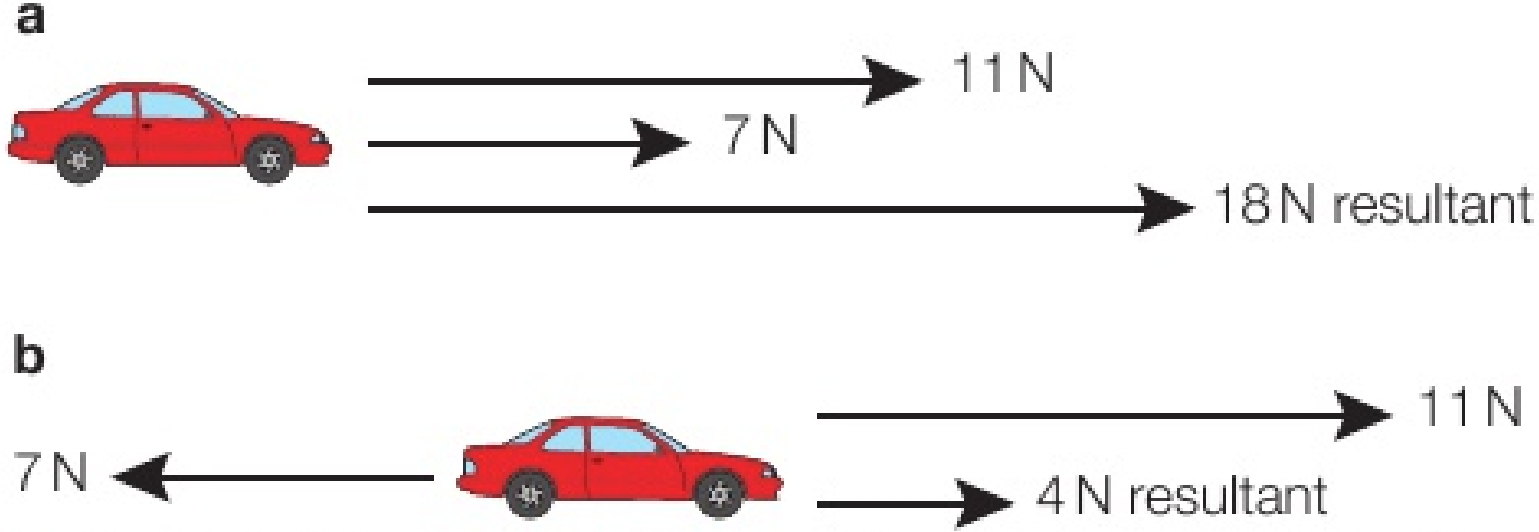
\includegraphics[scale=0.15]{Physics/1A/Images/1A-3-1.png}
        \caption{Adding forces in the same line requires a consideration of their comparative directions.}
    \end{figure}
    \item \textbf{Resultant of perpendicular forces:} For two forces at right angles, use Pythagoras to find the magnitude of
    the resultant:
    \begin{equation}
        F = \sqrt{F_x^2 + F_y^2}
    \end{equation}
    where $F_x$ and $F_y$ are the component forces. The direction (angle $\theta$ of $F$ from one axis) can be found by:
    \begin{equation}
        \tan \theta = \frac{F_y}{F_x}
    \end{equation}
    \begin{center}
        \begin{tikzpicture}
            \draw[->] (0,0) -- (5,0) node[below] {$F_x$};
            \draw[->] (0,0) -- (0,4) node[left] {$F_y$};
            \draw[->] (0,0) -- (5,4) node[above right] {$F$};
            \draw (0.5,0) -- (0.5,0.5) -- (0,0.5);
            \node at (0.7,0.3) {$\theta$};
            \draw (1,0) arc[start angle=0,end angle=38,radius=1cm];
        \end{tikzpicture}
    \end{center}
    \item \textbf{Parallelogram rule (vector addition):} For two forces at any angle, draw them to scale from the same point;
    complete the parallelogram - the diagonal from the common start point gives the resultant in magnitude and direction.
\end{itemize}

\paragraph{Theoretical Concepts}
\begin{itemize}
    \item \textbf{Combining Forces in the Same Line:} When forces act \underline{collinearly} (共线, along the same straight line),
    simply add or subtract their magnitudes with proper sign. Forces in the same direction \underline{reinforce} (加强) each other
    (add up), while forces in opposite directions \underline{counteract} (抵消) each other (subtract).
    \item \textbf{Combining Perpendicular Forces:} Forces acting at right angles (perpendicular) to each other can be combined
    using geometry. Draw the two force vectors as perpendicular arrows from a common point (forming a right triangle with the
    resultant as the \underline{hypotenuse} (斜边)). The magnitude of the resultant can be found by Pythagoras' theorem:
    \begin{equation}
        F = \sqrt{F_x^2 + F_y^2}
    \end{equation}
    The direction of the resultant can be found with \underline{trigonometry} (三角函数): for example \footnote{\textbf{Arctan}
    (or inverse tangent, denoted as $\tan^{-1} x$ or $\arctan x$) is the inverse function of the tangent function. It returns
    the angle $\theta$ in radians whose tangent $x$ is, typically within the principal range
    $-\frac{\pi}{2} \leq \theta \leq \frac{\pi}{2}$.},
    \begin{equation}
        \theta = \tan^{-1} \left( \frac{F_y}{F_x} \right) \quad \text{or} \quad \theta = \arctan \left( \frac{F_y}{F_x} \right)
    \end{equation}
    specifying $\theta$ as the angle relative to one of the original force directions. Always state the reference direction for
    the angle (e.g., $\theta$ above the horizontal) for clarity. \par
    \textbf{Exam Tip:} Always carefully state where the angle is measured from (this is best shown on a diagram).
\end{itemize}

\paragraph{Combining Forces at Angles - Parallelogram Rule}
When forces are not perpendicular and we need the resultant, we can use a scale diagram method (parallelogram rule). Draw both
force vectors from the same point to scale (same scale for both) at the correct angle between them. Then draw parallels to each
vector from the tip of each other, forming a parallelogram. The \underline{diagonal} (对角线) of the parallelogram from the common
start point represents the resultant force in both magnitude and direction. \par
This graphical method is often used in exams if an analytical method is not required or when forces are at awkward angles. If we
know how to use trigonometry for non-$90^\circ$ cases, that's fine, but follow the question's instructions - if it asks for a scale
drawing, use that approach. to get full marks.
\begin{figure}[H]
    \centering
    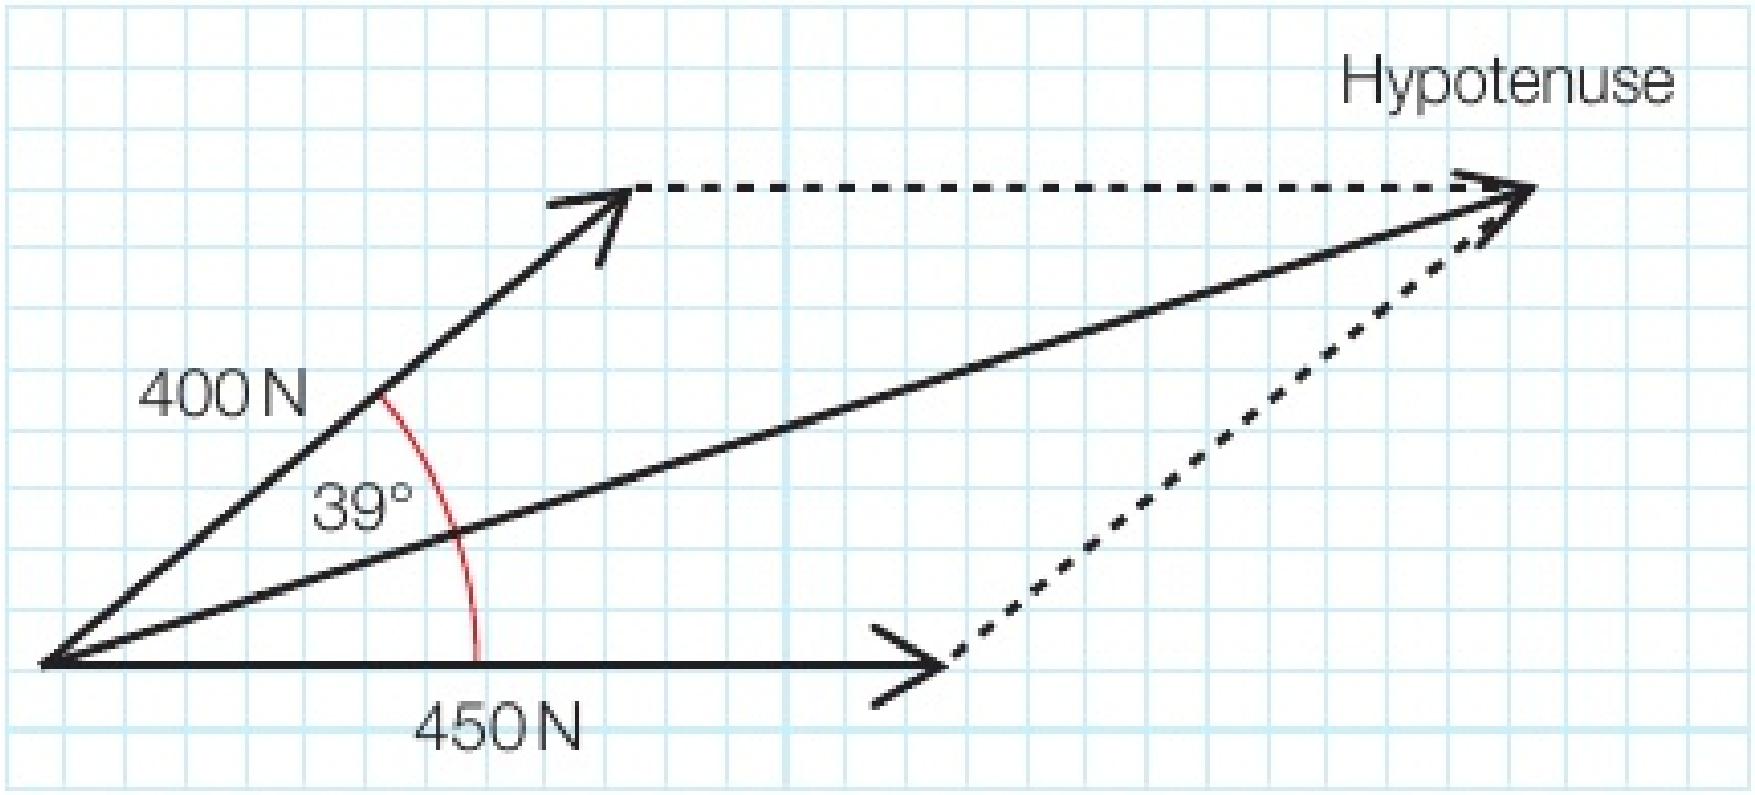
\includegraphics[scale=0.1]{Physics/1A/Images/1A-3-2.png}
    \caption{Finding the resultant vector using the parallelogram rule.}
\end{figure}

\paragraph{\underline{Co-Planar Forces} (共面力) and Multiple Vectors}
The \underline{vector-addition methods} (向量加法) above (triangles or parallelograms) work for any vectors as long as they are
co-planar (lying in the same plane). In most mechanics problems, forces are co-planar (e.g., acting in a 2D plane like a flat
diagram). \par
If more than two forces are present, we can add them one by one: first find the resultant of two forces, then add that resultant
to the next force, and so on. For multiple forces on different lines, it's often easiest to break them into components along
perpendicular axes (resolution of vectors) and sum all components in each direction.

\paragraph{\underline{Free-Body Force Diagrams} (受力分析图)}
A free-body force diagram is crucial tool for visualizing forces. In free-body diagram, we draw the object (often as a dot or a
simple box) isolated from its surroundings, and then draw all the forces acting on that object as arrows pointing in the
direction each force is applied. Each arrow's length should be drawn to scale relative to the force's magnitude (when possible),
and it should be labeled with the force value or name. \par
Forces \underline{exerted} (施加) by the object on others or forces on other objects are not included - only forces acting on the
chosen object. Free-body diagrams help in applying Newton's laws \footnote{\textbf{Newton's Laws of Motion}
\begin{itemize}
    \item \textbf{\underline{Newton's First Law} (牛顿第一定律 / 惯性定律, Law of Inertia):} An object at rest stays at rest, and an
    an object in motion stays in motion with the same velocity unless acted upon by an external force. This means that in the
    \underline{absence} (缺乏) of an unbalanced force, and object will maintain its current state of motion.
    \item \textbf{\underline{Newton's Second Law} (牛顿第二定律 / 动力定律, Law of Acceleration):} The acceleration of an object is
    directly proportional to the net force acting on it and inversely proportional to its mass, given by the equation:
    \begin{equation*}
        F = ma
    \end{equation*}
    where $F$ is the net force (in Newtons), $m$ is the object's mass (in kg), and $a$ is the acceleration (in m/$\text{s}^2$).
    This law explains how forces affect motion.
    \item \textbf{\underline{Newton's Third Law} (牛顿第三定律 / 作用与反作用定律, Law of Action-Reaction):} For every action, there
    is an equal and opposite reaction. This means that whenever one object \underline{exerts} (施加) a force on another, the
    second object exerts an equal force in the opposite direction on the first object.
\end{itemize}} or in setting up \underline{equilibrium equations} (平衡方程) by clearly showing all forces for vector addition.
\begin{figure}[H]
    \centering
    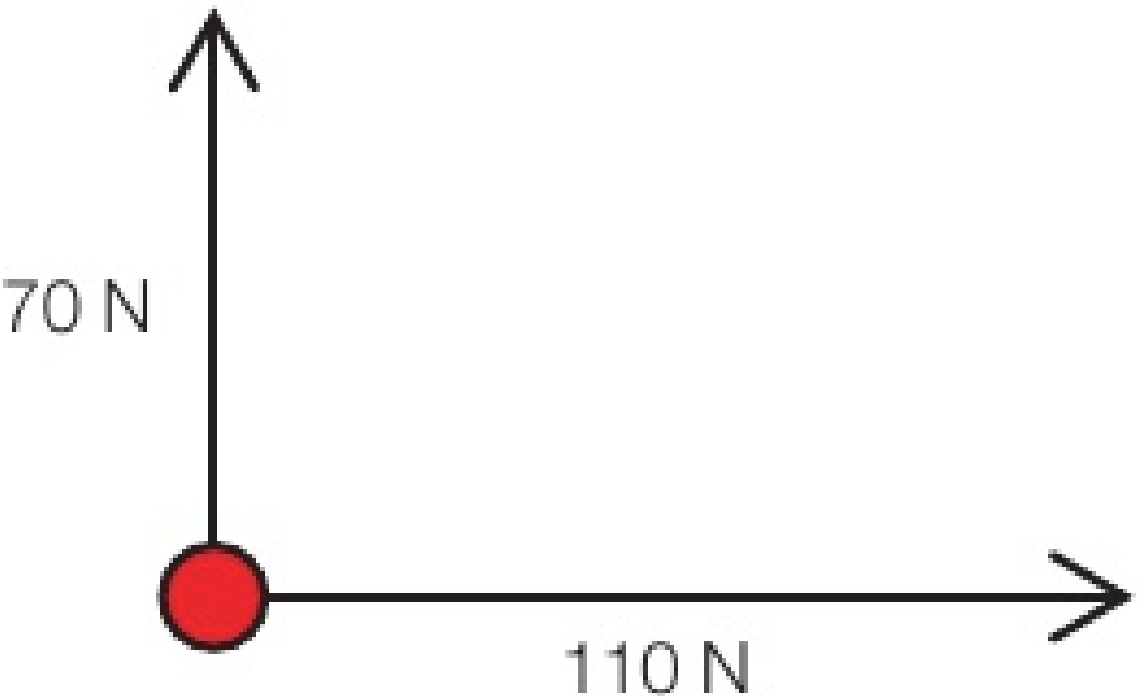
\includegraphics[scale=0.1]{Physics/1A/Images/1A-3-3.png}
    \caption{Free-body force diagram of a rugby player (red circle). The forces from the tacklers are marked on as force arrows.}
\end{figure}

\paragraph{Exam Tips}
\begin{itemize}
    \item \textbf{Indicate Directions:} Always indicate the direction of resultant force (e.g., '18N to the right' or 'Resultant
    = 5N at $30^\circ$ above the horizontal'). \underline{Merely} (仅仅只是) giving a magnitude is not \underline{sufficient}
    (足够的) for full marks.
    \item \textbf{State Angle Reference:} When giving an angle for a resultant, state what it's measured from (horizontal,
    vertical, etc.). This avoids \underline{ambiguity} (模棱两可) in answers.
    \item \textbf{Use Scale Drawings Correctly:} If a question specifies a scale drawing or the parallelogram / triangle method,
    do so. Use a ruler for straight lines and a protector for angles to ensure accuracy. Label the scale (e.g., '1cm = 10N'). In
    calculation questions, directly use trig and Pythagoras, but still draw a quick diagram to guide the work.
    \item \textbf{Co-Planar Assumption:} All these addition methods assume forces lie in the same plane. This is usually the case
    in exam problems. If forces are not co-planar (rare at this level), you would handle one plane at a time or resolve into
    components in 3D - but typically stick to 2D planes.
    \item \textbf{Add \underline{Iteratively} (反复 \ 迭代) for Many Forces:} When more than two forces act, add them
    \underline{stepwise} (逐步地). Combine two into a resultant, then combine that resultant with the next force, etc. This
    \underline{incremental} (递增的) approach reduces confusion and is less \underline{error-prone} (易错) than trying to do all
    at once.
    \item \textbf{Check Equilibrium Conditions:} If the question implies an object is in equilibrium (not accelerating), the
    resultant force should come out to zero. Use this as a check: forces should balance out in all directions. A common exam
    trick is to have forces that cancel out; recognizing equilibrium can simplify the problem.
\end{itemize}